\section{Related Work}

Convolutional networks have become popular in large scale image recognition
tasks after Krizhevsky et al.~\cite{krizhevsky2012imagenet}. Some of the next important
milestones were Network-in-network~\cite{lin2013network} by Lin et al.,
VGGNet~\cite{simonyan2014very} by Simonyan et al. and GoogLeNet
(Inception-v1)~\cite{szegedy2015going} by Szegedy et al.

Residual connection were introduced by He et al. in~\cite{he2015deep} in
which they give convincing theoretical and practical evidence for the
advantages of utilizing additive merging of signals both for image recognition, and especially for object detection.
The authors argue that residual connections are inherently necessary for training
very deep convolutional models. Our findings do not seem to support this
view, at least for image recognition. However it might require more
measurement points with deeper architectures to understand the true extent
of beneficial aspects offered by residual connections.
In the experimental section we demonstrate that it is not very difficult to
train competitive very deep networks without utilizing residual connections.
However the use of residual connections seems to improve the training speed
greatly, which is alone a great argument for their use.
\begin{figure}
\centering
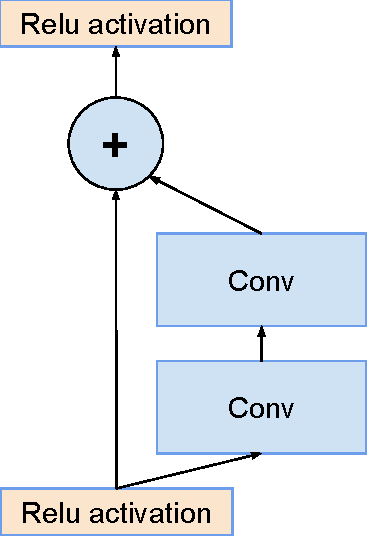
\includegraphics[width=0.5\linewidth]{resnetsimple}
\caption{Residual connections as introduced in He et al.~\cite{he2015deep}.}
\label{fig:resnetsimple}
\end{figure}
\begin{figure}
\centering
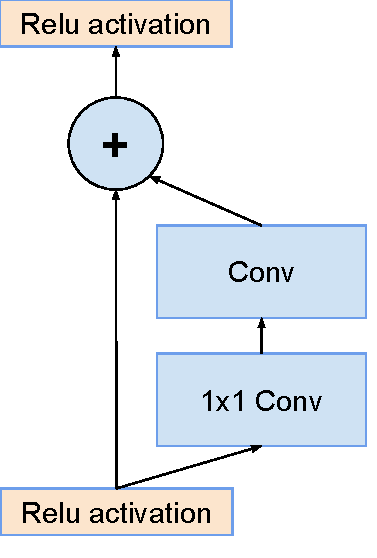
\includegraphics[width=0.5\linewidth]{resnetoptimized}
\caption{Optimized version of ResNet connections by~\cite{he2015deep} to
  shield computation.}
\label{fig:resnetoptimized}
\end{figure}
The Inception deep convolutional architecture was introduced
in~\cite{szegedy2015going} and was called GoogLeNet or Inception-v1 in our
exposition.
Later the Inception architecture was refined in various ways,
first by the introduction of batch normalization
~\cite{ioffe2015batch} (Inception-v2) by Ioffe et al.
Later the architecture was improved by additional factorization ideas in the
third iteration~\cite{szegedy2015rethinking} which will be referred to as
Inception-v3 in this report.
